\documentclass[11pt,reqno,oneside]{article}
% \documentclass[12pt, final]{siamonline171218}
% \usepackage[pdfborder={0 0 0.5 [3 2]}]{hyperref}%
\usepackage[left=1in,right=1in,top=1in,bottom=1in]{geometry}%
\usepackage{amsmath}
\usepackage{amssymb}
\usepackage{amsthm}
\usepackage{graphicx}
\usepackage{enumerate}
\usepackage{float}
\usepackage{bm}
\usepackage[stable]{footmisc}

\usepackage{packages}
\usepackage{wrapfig}
\usepackage{subfigure}
\usepackage[font=footnotesize]{caption}

\newtheorem{theorem}{Theorem}
\newtheorem{lemma}[theorem]{Lemma}
\newtheorem{corollary}{Corollary}

\theoremstyle{definition}
\newtheorem{definition}[theorem]{Definition}

\theoremstyle{remark}
\newtheorem{remark}[theorem]{Remark}

\def\noi{\noindent}
\def\T{{\mathbb T}}
\def\R{{\mathbb R}}
\def\N{{\mathbb N}}
\def\Z{{\mathbb Z}}
\def\C{{\mathbb C}}
\def\Q{\mathbb{Q}}

\newcommand{\vK}{\bm{\mathit{K}}}
\newcommand{\calP}{\mathcal{P}}
\newcommand{\calA}{\mathcal{A}}

\newcommand{\xvec}{\mathbf{x}}

\setlength{\parindent}{0em}
\setlength{\parskip}{1em}
\renewcommand{\baselinestretch}{1.1}

\title{Research Statement}
\date{\vspace{-12ex}}

\begin{document}

\thispagestyle{empty}

% \maketitle

\subsection*{Research Summary}

My main research focus is on understanding patterns and coherent structures arising in the natural sciences and engineering. Mathematically, these are described by nonlinear evolution equations, which take the form of partial differential equations (PDEs) or systems of ordinary differential equations (ODEs). Most of the systems I study are nonlinear wave equations, which describe the time evolution of a function representing a wave profile. Coherent structures are spatial patterns which maintain their shape as the system evolves in time. 
Examples of coherent structures include solitary waves, which are localized disturbances that propagate at a constant velocity; wavetrains, which are periodic disturbances that also propagate at a constant velocity; and breathers, which are disturbances that are localized in space but oscillate in time. 
Solitary waves have been a topic of interest since the 19th century, when John Scott Russell observed a single, large surface wave on the Edinburgh-Glasgow Union Canal in Scotland; the wave propagated along the canal undisturbed for a few miles before eventually decaying. 
This phenomenon was explained mathematically by the Korteweg–de Vries (KdV) equation 
\[
u_t + u_{xxx} + 6 u u_x = 0,
\]
which has both solitary wave and wavetrain solutions.
\begin{figure}[H]
    \centering
    \begin{tabular}{cc}
        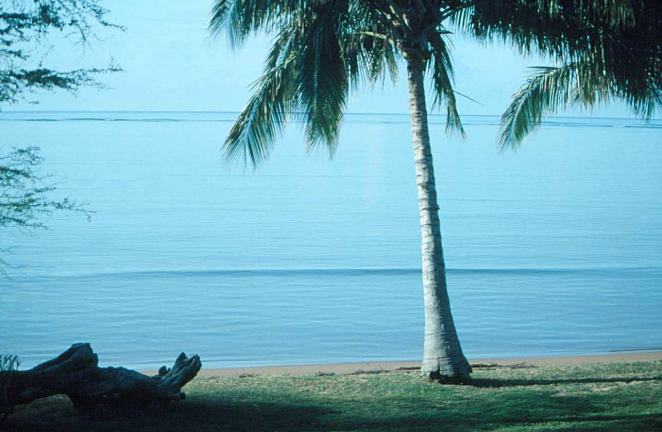
\includegraphics[width=7cm]{images/SolitaryWaveHawaii.png} &
        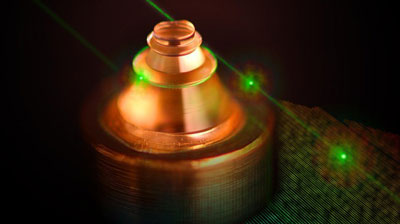
\includegraphics[width=8.1cm]{images/resonator.jpg}      
    \end{tabular}
    \caption{Solitary wave off the coast of Hawaii \cite{Andriopoulos2009} (left). Optical solitons in a microresonator \cite{MarinPalomo2017} (right) }
    \label{fig:solitarywaves}
\end{figure}
Although solitary waves were originally discovered as a water wave phenomenon, they have applications in many fields, including fiber optics, plasma physics, quantum mechanics, molecular biology, and neuroscience (\cref{fig:solitarywaves}). More generally, many nonlinear, dispersive PDEs exhibit solitary wave solutions. My research falls into two broad categories. First, I study the existence and spectral stability of complex structures in Hamiltonian systems; these systems are characterized by a conserved quantity, such as energy, that remains constant in time. These patterns are constructed using simpler objects, such as solitary waves, as building blocks. 
Second, I study localized patterns in lattices of optical fibers, using mathematical models which are inspired by recent advances in experimental optics. Finally, some very recent work explores bifurcation structures in neural network models in the presence of symmetries in the connectivity matrix describing the network.

\subsection*{Coherent structures in Hamiltonian systems}

The bulk of my published research concerns coherent structures in Hamiltonian systems. At a high level, I start with a simple coherent structure, such as a solitary wave, and use it as a building block to construct more elaborate structures. I then study the stability of these more complicated structures in terms of their underlying geometry, together with properties of the simpler structure. 

The prototypical nonlinear wave equation has a primary solitary wave solution, also known as a primary pulse solution, which looks like a single localized ``bump'' (\cref{fig:linsmethod}, left). In many systems, multi-pulse solutions also exist; these are ``multi-bump'' solitary waves, which resemble a sequence of multiple, well-separated copies of the primary pulse. The entire multi-pulse structure travels as a unit, and it maintains its shape unless perturbed. In addition to having applications in nonlinear optics and neuroscience, multi-pulses are interesting mathematically. In my research, I explore the existence and stability of these multi-pulse structures. A crucial step in this process is determining the spectrum of the linearization of the underlying system about a multi-pulse. When a multi-pulse is perturbed, interactions between the individual pulses in the structure are revealed, which are a consequence of the inherent nonlinearity of the system. The dynamics of these interactions are determined by the eigenvalues of the linearized system and their corresponding eigenfunctions.

\begin{figure}
    \centering
    \begin{tabular}{cc}
        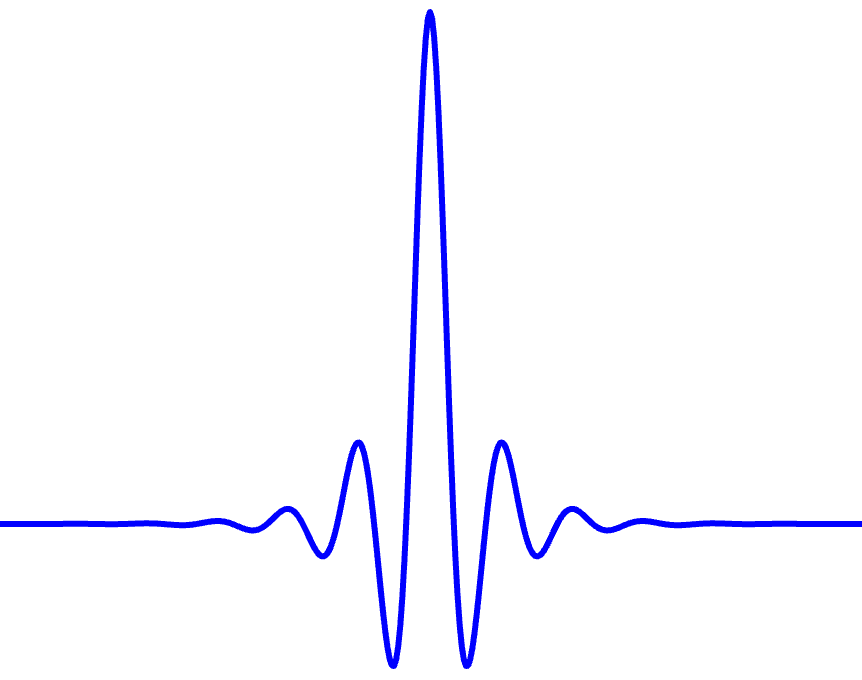
\includegraphics[width=4.5cm]{images/linchen1.png} &
        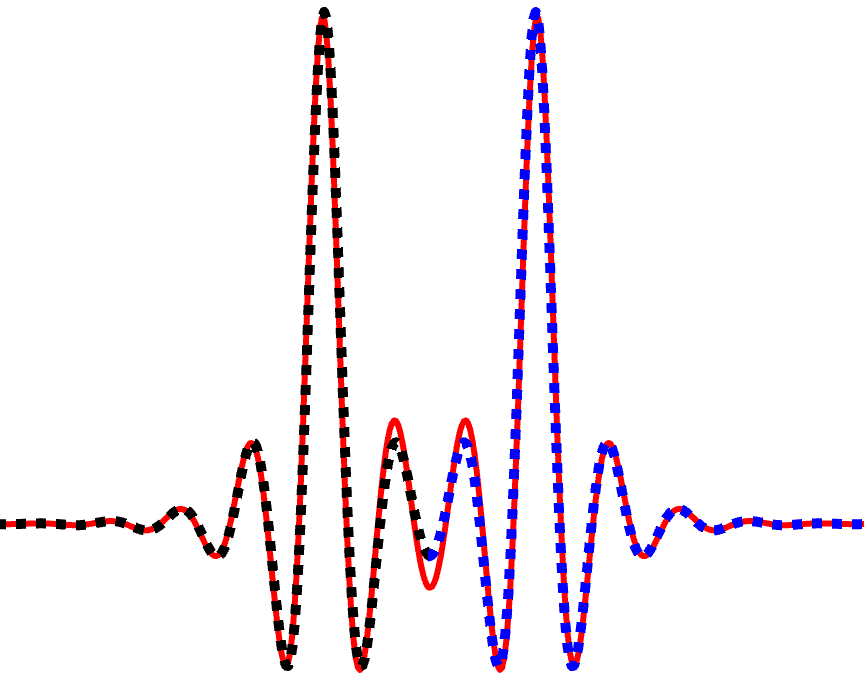
\includegraphics[width=4.5cm]{images/linchen2.png} 
    \end{tabular}
    \caption{Cartoon illustrating construction of a double pulse solution using Lin's method. Left panel shows primary pulse solution. Right panel shows two copies of the primary pulse solution (black and blue dotted lines) placed end-to-end. Double pulse solution (red solid line) is close, but not equal, to this.}
    \label{fig:linsmethod}
\end{figure}

My primary mathematical approach comes from spatial dynamics. From this viewpoint, a solitary wave is a homoclinic orbit evolving in the spatial variable $x$. For example, the solitary wave solution $u(x)$ to the KdV equation which travels to the right with constant speed $c$ (\cref{fig:kdvpp}, left) is a solution to the second order ODE 
\[
u_{xx} + 3 u^2 - c u = 0.
\]
This can be written as the two-dimensional dynamical system 
\[
\frac{d}{dx}\begin{pmatrix}u\\v\end{pmatrix}
= \begin{pmatrix}v \\ cu - 3u^2\end{pmatrix}
\]
by taking $v = u_x$. From this perspective, the solitary wave solution $(u(x), v(x))$ is a homoclinic orbit connecting the unstable and stable manifolds of the saddle equilibrium point at the origin (\cref{fig:kdvpp}, right), which represents the rest state of the system. 

\begin{figure}
    \centering
    \begin{tabular}{cc}
        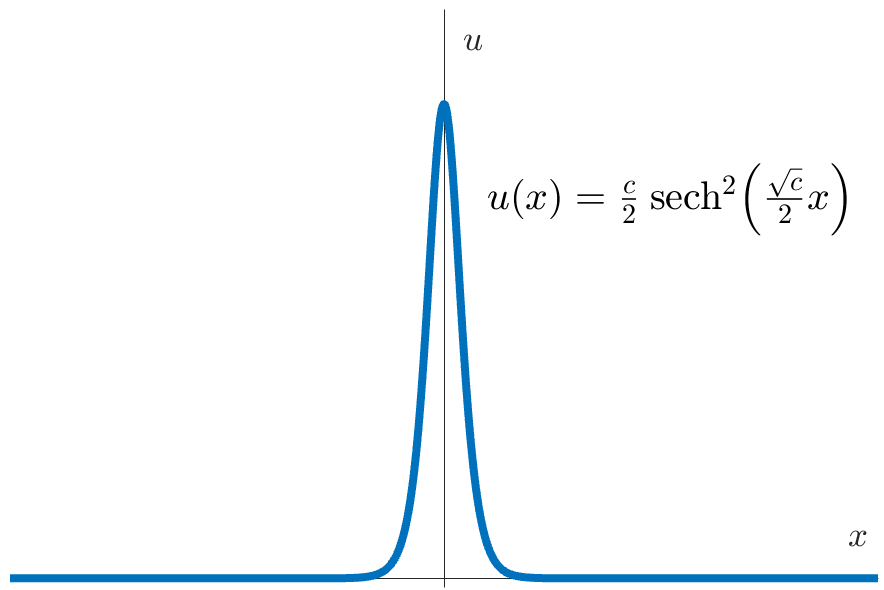
\includegraphics[width=6cm]{images/KdVsolitoneq.png} \hspace{2cm} &
        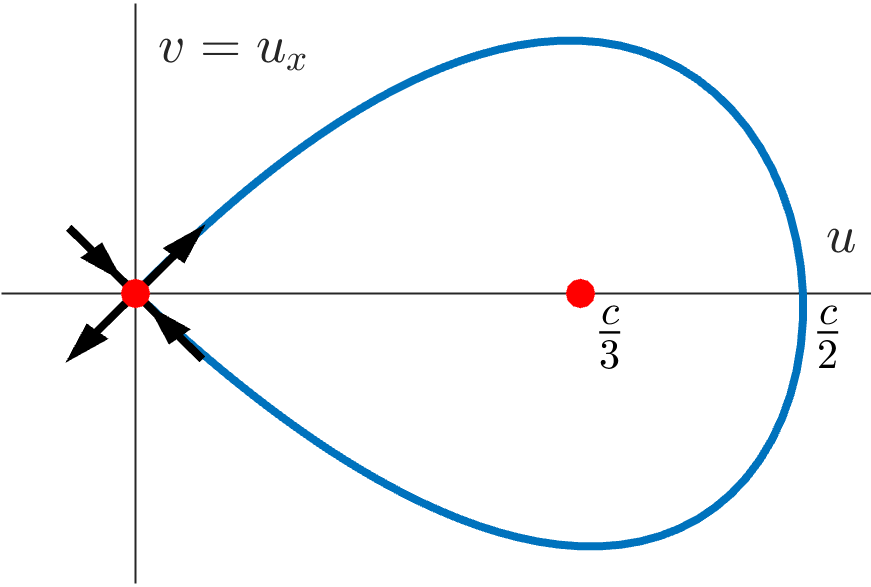
\includegraphics[width=6cm]{images/KdVphaseportait.png} 
    \end{tabular}
    \caption{Primary solitary wave solution $u(x)$ to the KdV equation. Left panel is plot of $u$ vs $x$. Right panel is plot of $u_x$ vs $u$, showing solitary wave as a homoclinic orbit.}
    \label{fig:kdvpp}
\end{figure}

From a spatial dynamics perspective, multi-pulses are multi-loop homoclinic orbits. (Notably, multi-pulses do not exist in the KdV equation, since the phase space for the primary homoclinic orbit is two-dimensional). Multi-pulses can be constructed using Lin's method \cite{Lin2008}, a version of the Lyapunov-Schmidt reduction, which can be used to find solutions that are close to a homoclinic orbit. Heuristically, this process involves ``gluing together'' multiple copies of the primary pulse solution end-to-end using small remainder functions (\cref{fig:linsmethod}, right). The existence of multi-pulse solutions is constrained by the geometry of the primary pulse and the underlying system. In \cref{fig:linsmethod}, for example, multi-pulses can only be constructed  when the tail oscillations of the individual pulses overlap in-phase. In general, each pulse that is added to a multi-pulse structure is associated with one or more eigenvalues in the spectrum of the linearized system, which I call interaction eigenvalues, since they result from nonlinear interactions between the tails of neighboring pulses. Since the systems I study are Hamiltonian, all eigenvalues must come in quartets of the form $\pm \alpha \pm \beta i$. Although this additional structure is helpful, it also means that the presence of any eigenvalue with nonzero real part implies that there is an unstable eigenvalue with positive real part. As a consequence, Hamiltonian systems cannot be dissipative, which makes stability analysis more difficult.
My main results relate the spectral pattern of the interaction eigenvalues to the underlying geometry of the multi-pulse. In all cases, the spectral pattern is determined by this geometry. 

\subsubsection*{Fifth-order KdV equation}

The fifth-order Korteweg de-Vries equation (KdV5) 
\[
\partial_t u - \partial_x^5 u + \partial_x^3 u + 2 u \partial_x u
\]
is a weakly nonlinear long wave approximation to the capillary-gravity wave problem, and also has applications to plasma physics and laser optics \cite{Pelinovsky2007}. Multi-pulse solutions to KdV5 exist \cite{SandstedeStrut}, but their stability analysis is complicated due to the fact that the essential spectrum for all localized solutions comprises the entire imaginary axis. In particular, this means that any purely imaginary interaction eigenvalues would be embedded in the essential spectrum, which makes them difficult to locate. To avoid this issue, I impose periodic boundary conditions on the problem, and look instead at multi-pulses on a periodic domain. As a consequence, the essential spectrum becomes a discrete set of eigenvalues on the imaginary axis (blue open circles in \cref{fig:periodic}, top right). Imaginary interaction eigenvalues can then lie between these essential spectrum eigenvalues, which avoids the problem of embedded eigenvalues. 

\begin{figure}
    \begin{center}
    \includegraphics[width=5cm]{images/2pulse3d.png}
    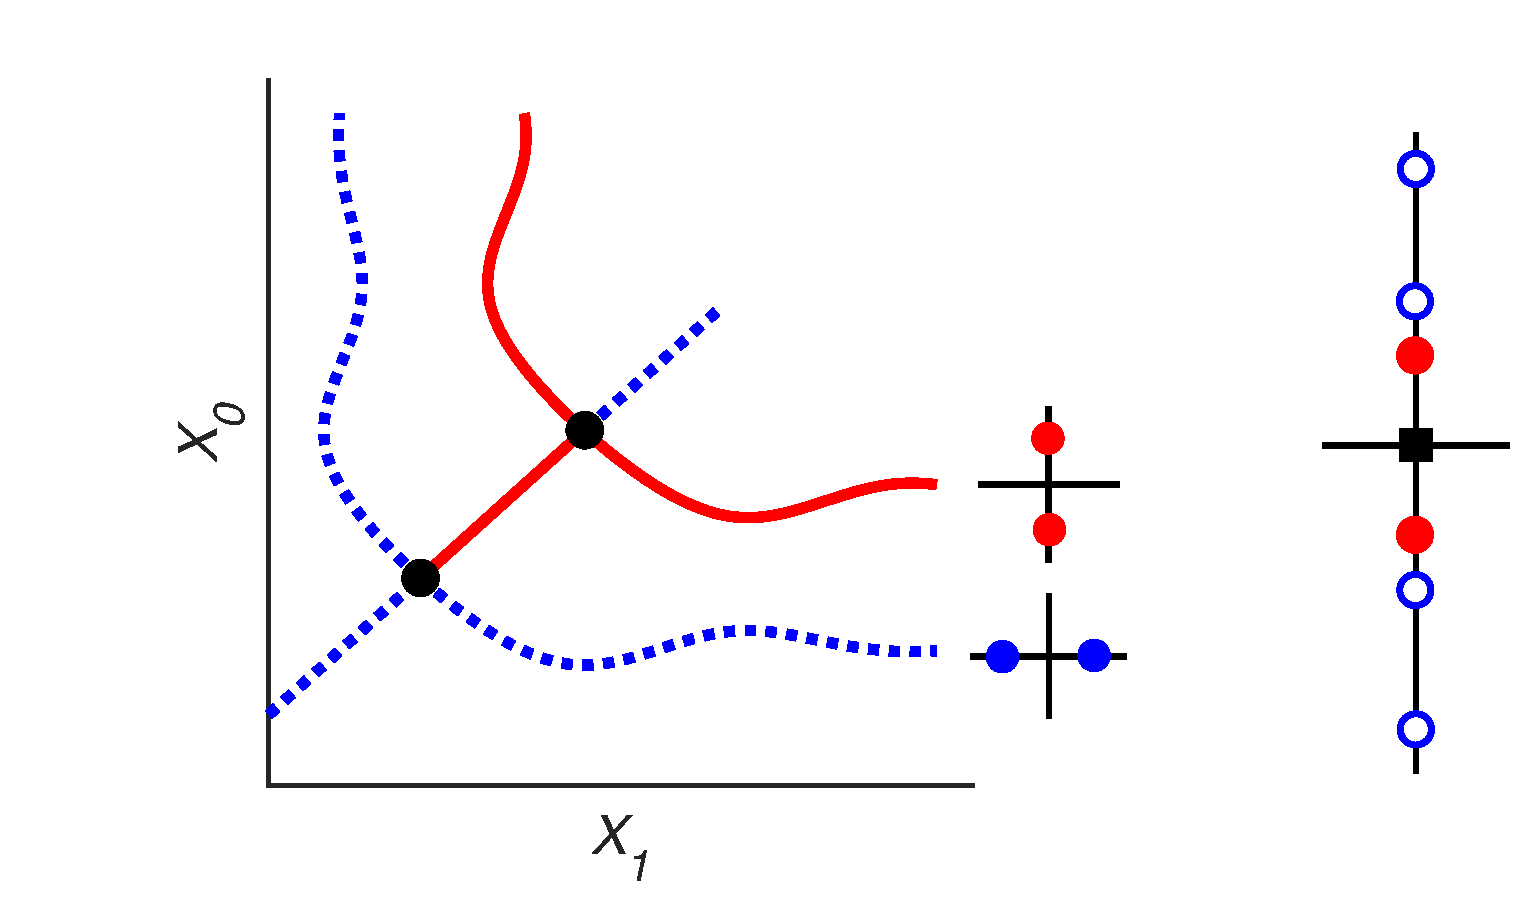
\includegraphics[width=7cm]{images/2pitchforkcoloreig2.eps}
    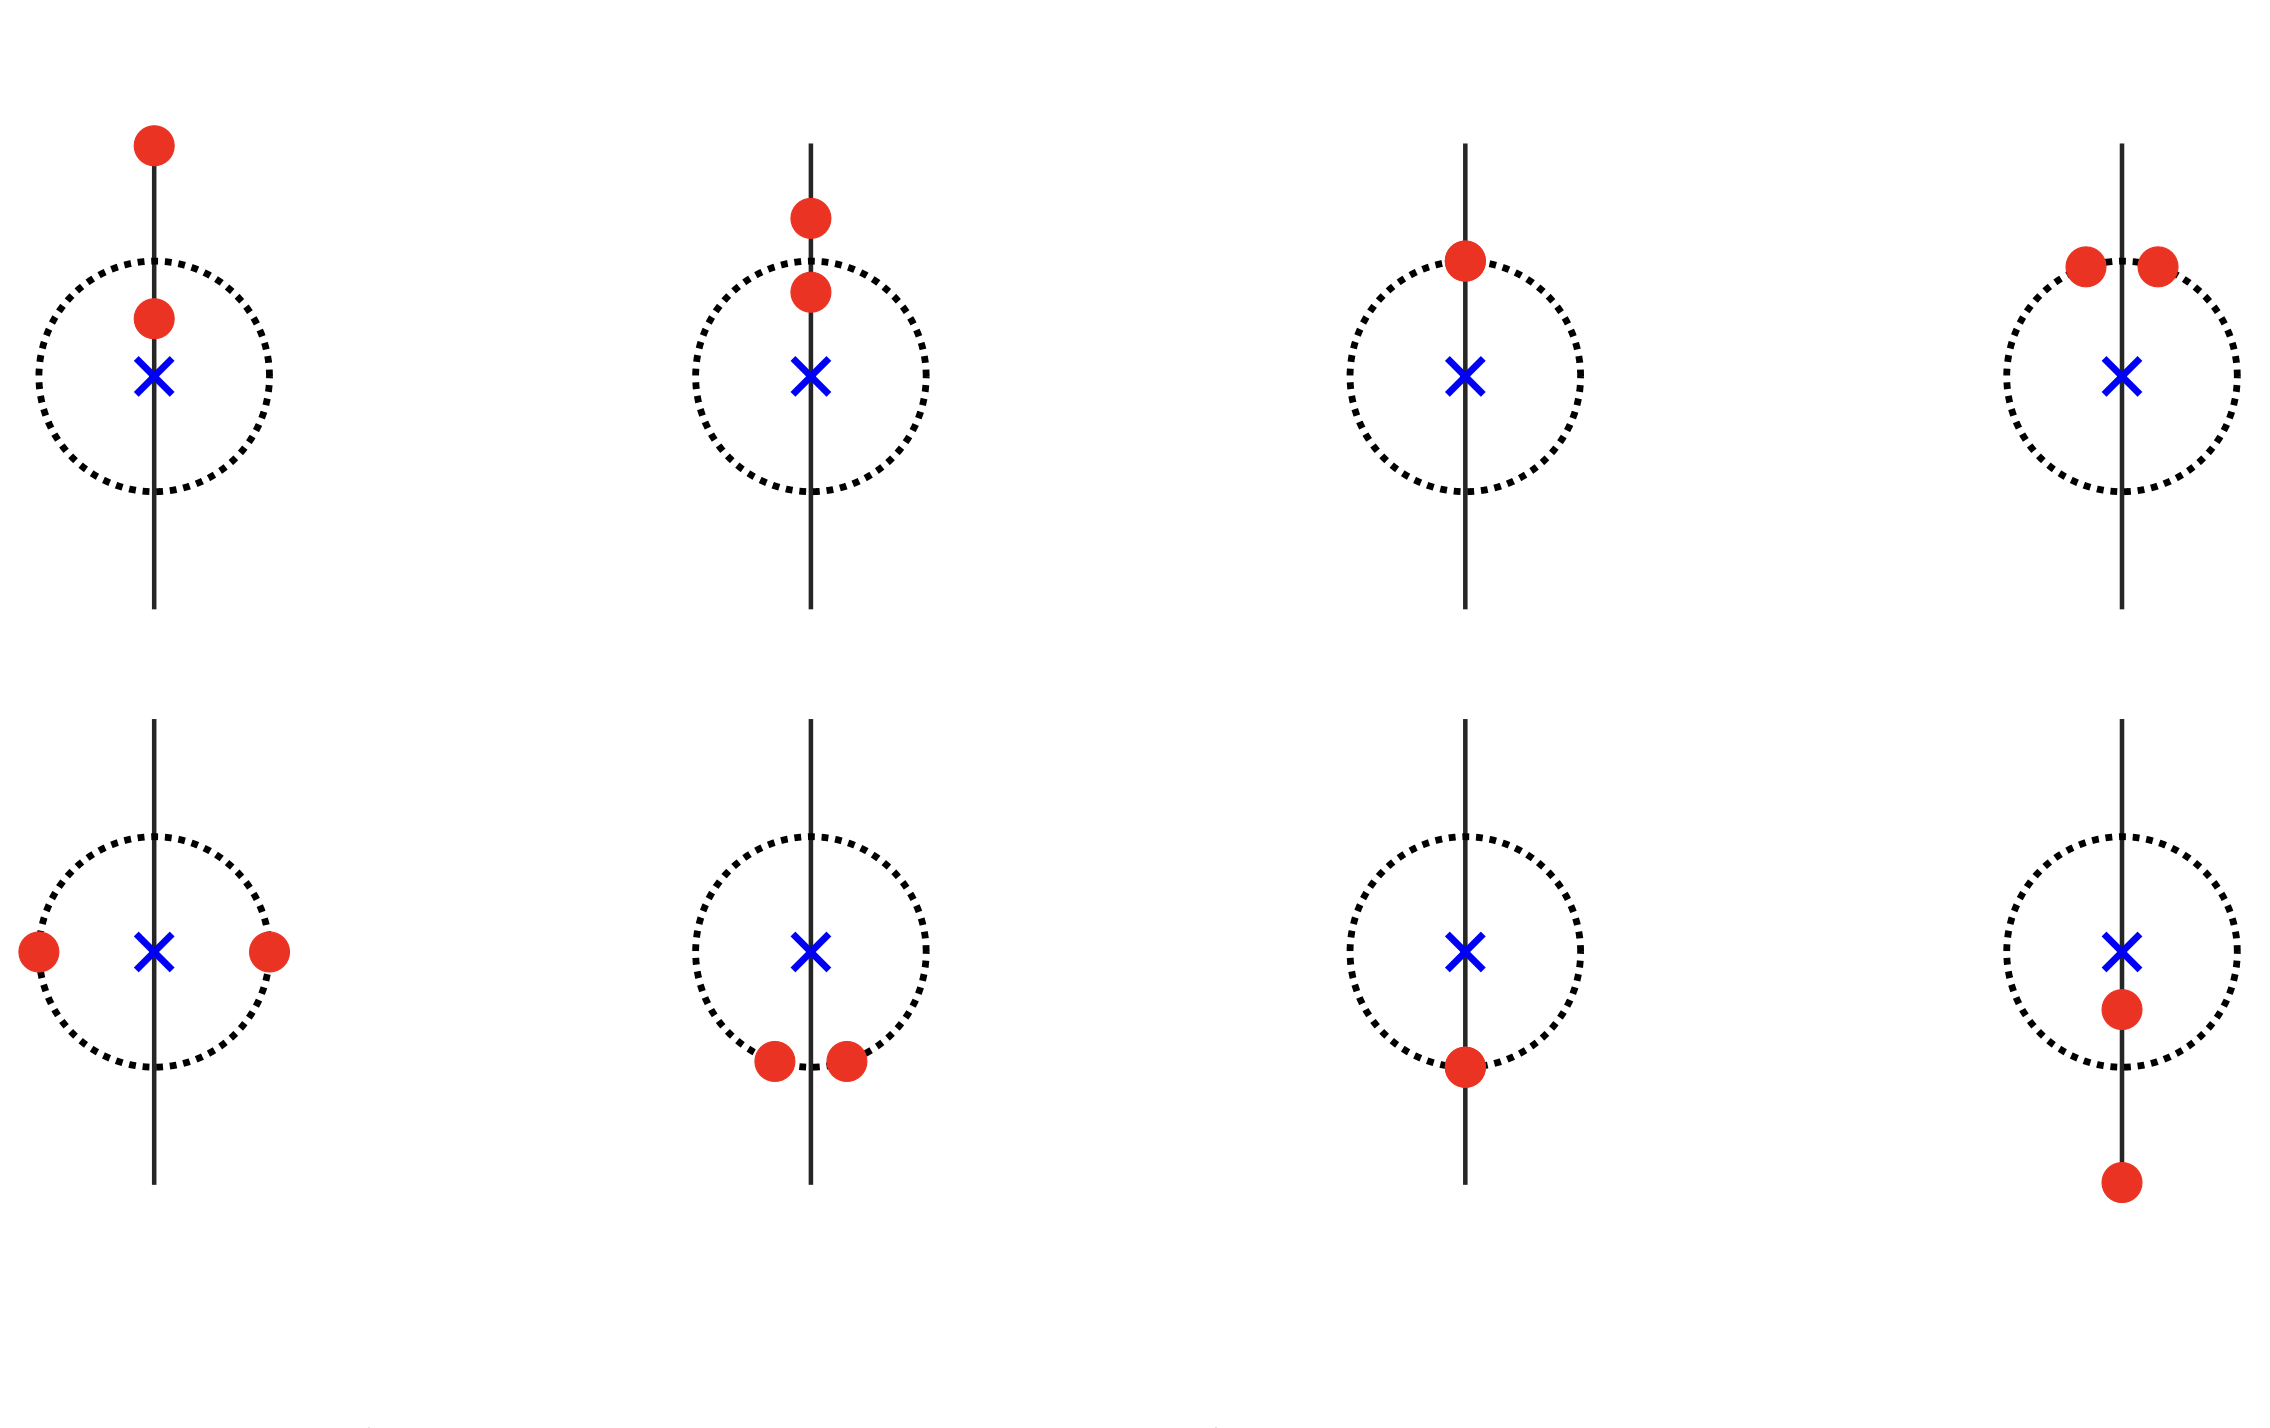
\includegraphics[width=8cm]{images/KreinBubbleCartoonSS2.png}
    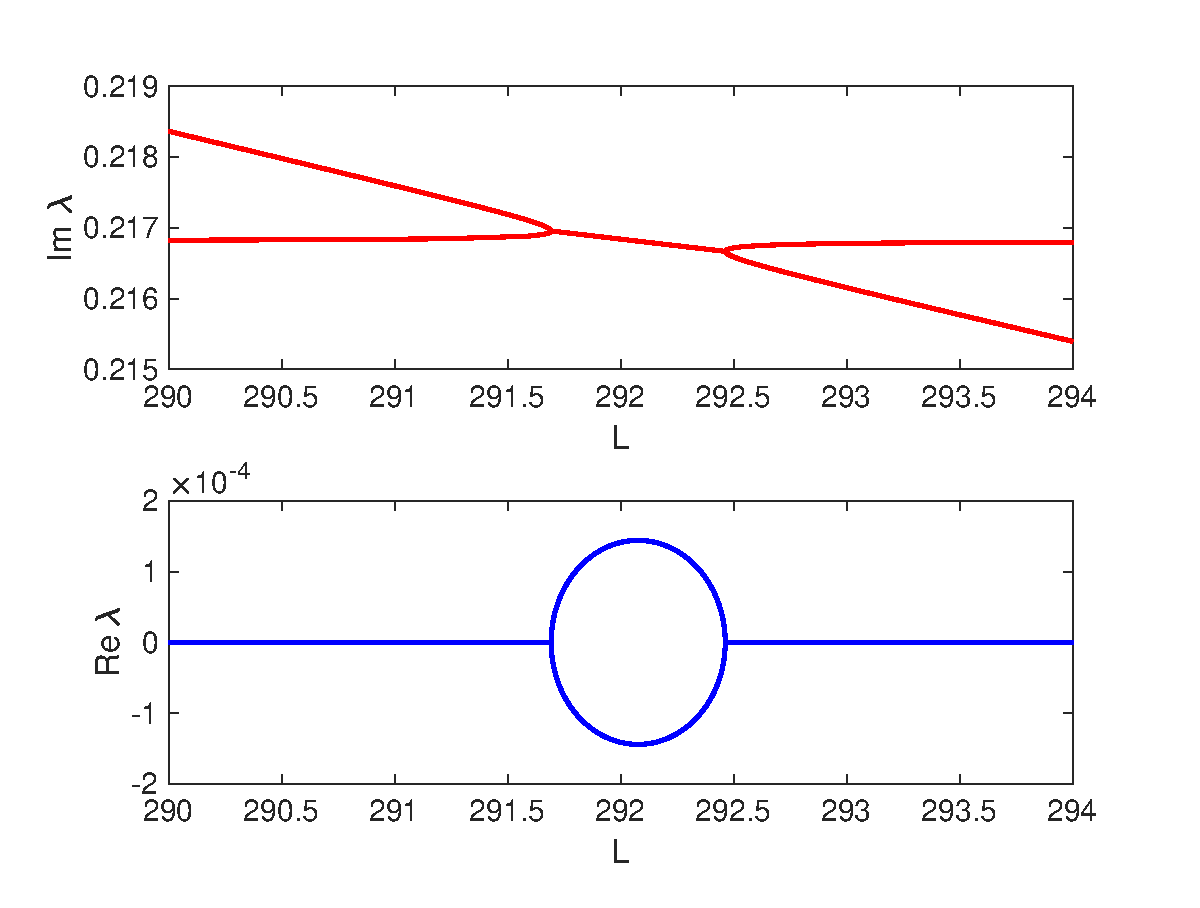
\includegraphics[width=7cm]{images/kreinbubble1.eps}
    \end{center}
    \caption{Top row: Construction (left) and bifurcation diagram with corresponding interaction eigenvalue pattern (center) of periodic double pulse solutions to KdV5. Spectrum of neutrally stable periodic double pulses (right) comprising interaction eigenvalues (red filled circles), essential spectrum eigenvalues (blue open circles), and kernel eigenvalue with algebraic multiplicity 2 (black square).
    Bottom row: schematic (left) and numerical simulation (right) of Krein instability bubble.}
    \label{fig:periodic}
\end{figure}

From a spatial dynamics perspective, periodic multi-pulses are multi-loop periodic orbits which lie close to the primary homoclinic orbit. These are constructed using Lin's method by ``gluing together'' multiple copies of the primary pulse end-to-end in a loop. A periodic double pulse is characterized by two length parameters $X_0$ and $X_1$ (\cref{fig:periodic}, top left), thus there is an extra degree of freedom when compared to a double pulses on the real line. As a consequence, periodic double pulses exist in a continuous family, in which asymmetric solutions (with $X_0 \neq X_1$) bifurcate from symmetric solutions (with $X_0 = X_1$) in a sequence of pitchfork bifurcations (\cref{fig:periodic}, top center) \cite{ParkerKdV}. Using Lin's method, I prove that the eigenvalues associated with a periodic multi-pulse can be found by solving a block matrix equation \cite[Theorem 5.3]{ParkerKdV}, which encodes both the interaction eigenvalues and eigenvalues associated with the essential spectrum. For periodic double pulses, there is a pair of interaction eigenvalues which is either real or imaginary, depending on the geometry of the solution (\cref{fig:periodic}, top center). The eigenvalue pattern switches between real and imaginary at the pitchfork bifurcation points. 

As the periodic domain size $X = X_0 + X_1$ is increased, the essential spectrum eigenvalues move towards the origin, while the interaction eigenvalues remain fixed (to leading order).
As $X$ passes through a critical value, there is a collision between an essential spectrum eigenvalue and a purely imaginary interaction eigenvalue, in which the two eigenvalues collide on the imaginary axis, move off the imaginary axis, trace an approximate circle in the complex plane, and recombine on the imaginary axis in a ``reverse'' collision (\cref{fig:periodic}, bottom left) \cite[Theorem 5.10]{ParkerKdV}. This brief instability bubble, which I call a Krein bubble since the eigenvalues involved in the collision have opposite Krein signatures, is a direct consequence of the block matrix reduction. A numerical simulation of the Krein bubble, computed using parameter continuation with the specialized software package AUTO, is shown in the bottom right of \cref{fig:periodic}. The location and size of the Krein bubble in the simulation agree with that predicted by the theory.

\subsubsection*{Fourth-order NLS equation}

The fourth-order generalization of the nonlinear Schr{\"o}dinger equation (NLS4)
\[
i u_t + \frac{\beta_4}{24}u_{xxxx} - \frac{\beta_2}{2}u_{xx} + \gamma |u|^2 u = 0
\]
was introduced to account for the role of small fourth-order dispersion terms in the propagation of intense laser beams in a bulk medium with Kerr nonlinearity \cite{Karpman2000,Tam2020}. Motivated by recent experiments \cite{Tam2019}, there is particular interest in the case where $\beta_2 = 0$, in which case the system exhibits pure quartic dispersion; the resulting solitary wave solutions are known as pure quartic solitons (PQS), which exist when $\beta_4 < 0$. I prove that while multi-pulse solitary wave solutions exist, they are all unstable due to the presence of at least one interaction eigenvalue with positive real part \cite[Theorems 1 and 2]{Parker2020NLS4}. The evolution of perturbations to these solutions can be explained by the interaction eigenvalues and their corresponding eigenfunctions.

\begin{figure}
    \begin{center}
    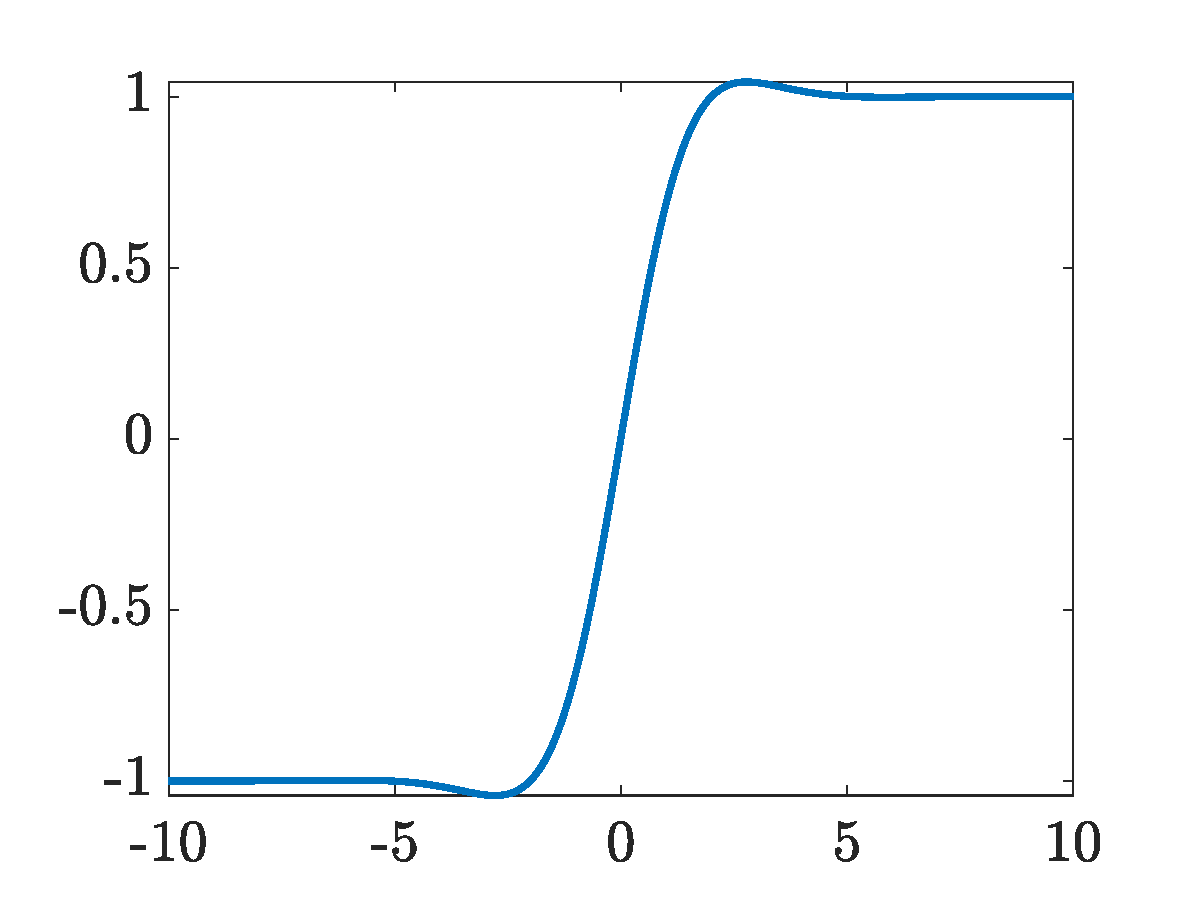
\includegraphics[width=5cm]{images/kink}
    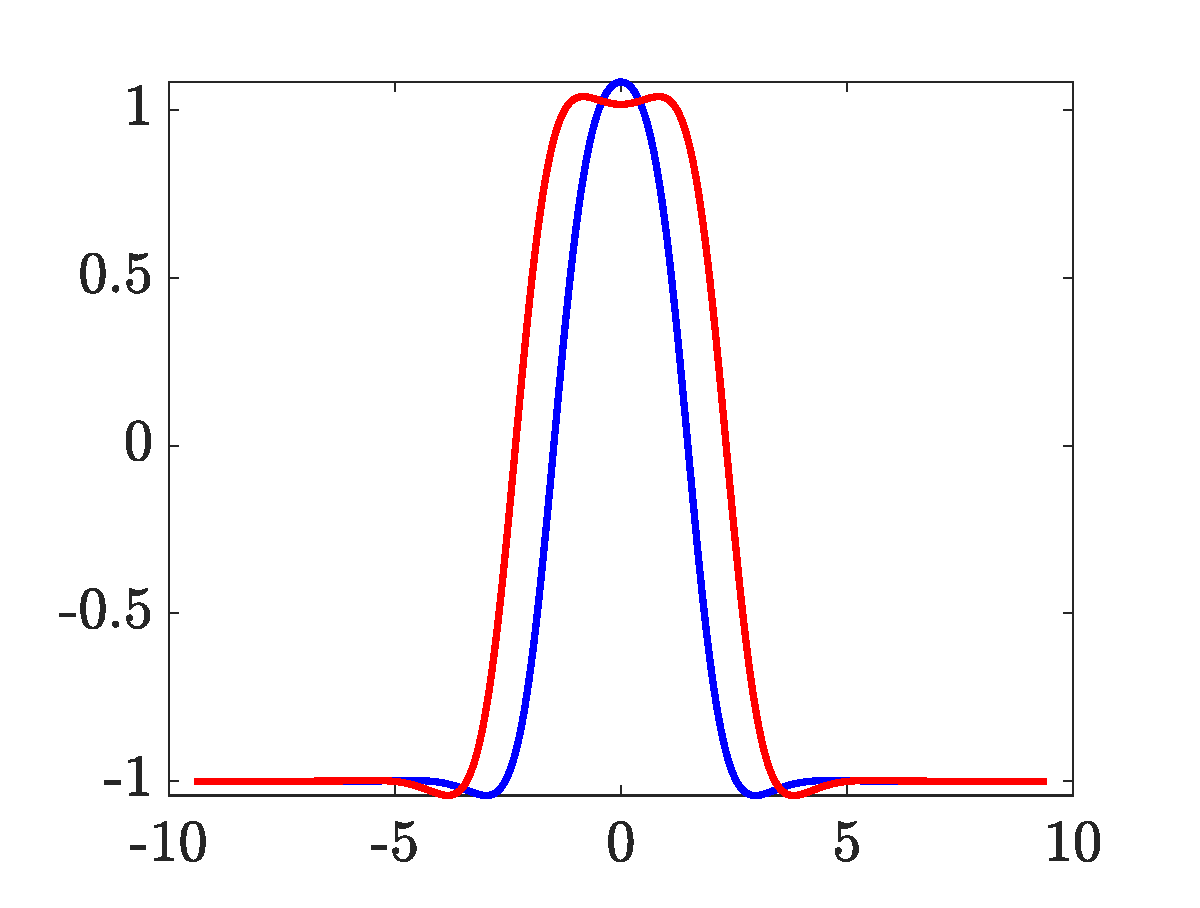
\includegraphics[width=5cm]{images/kak}\\
    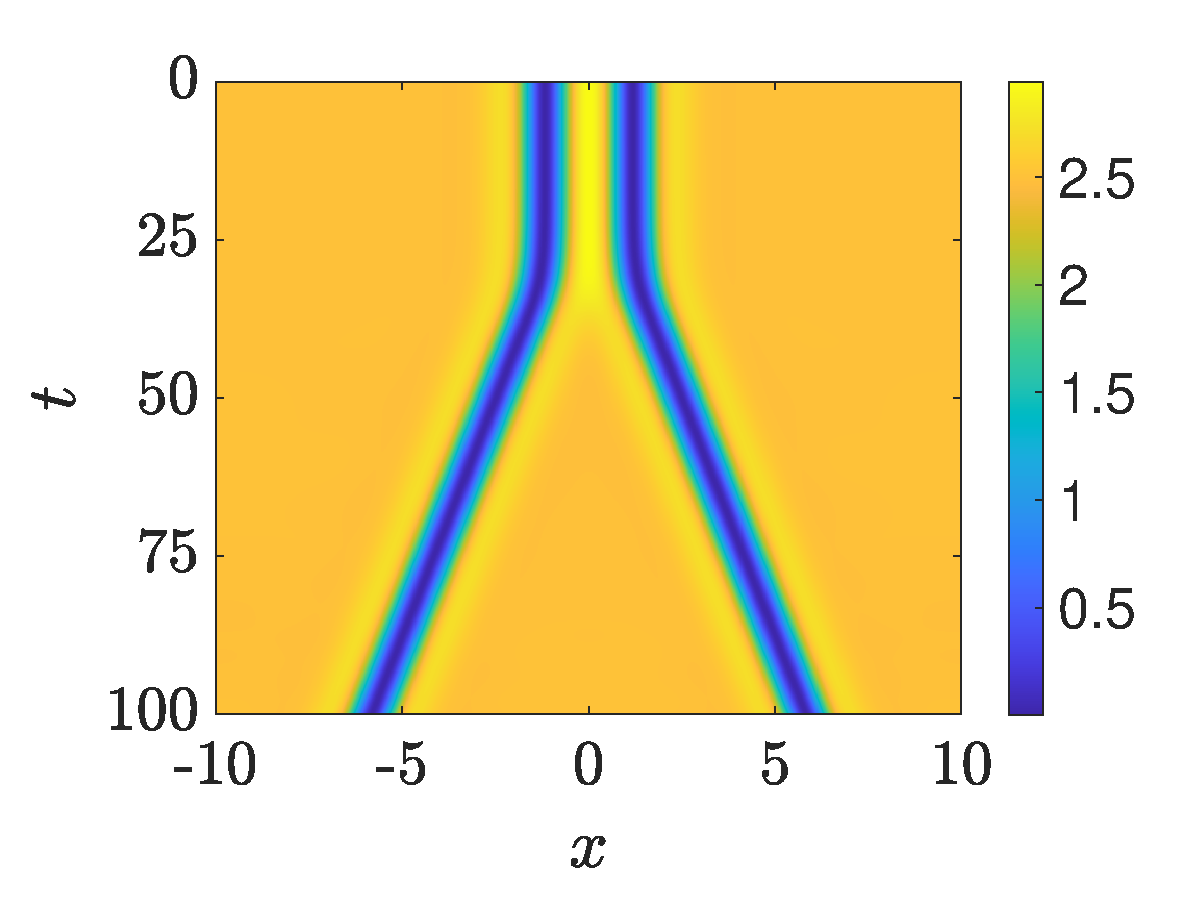
\includegraphics[width=5cm]{images/kak1colormap}
    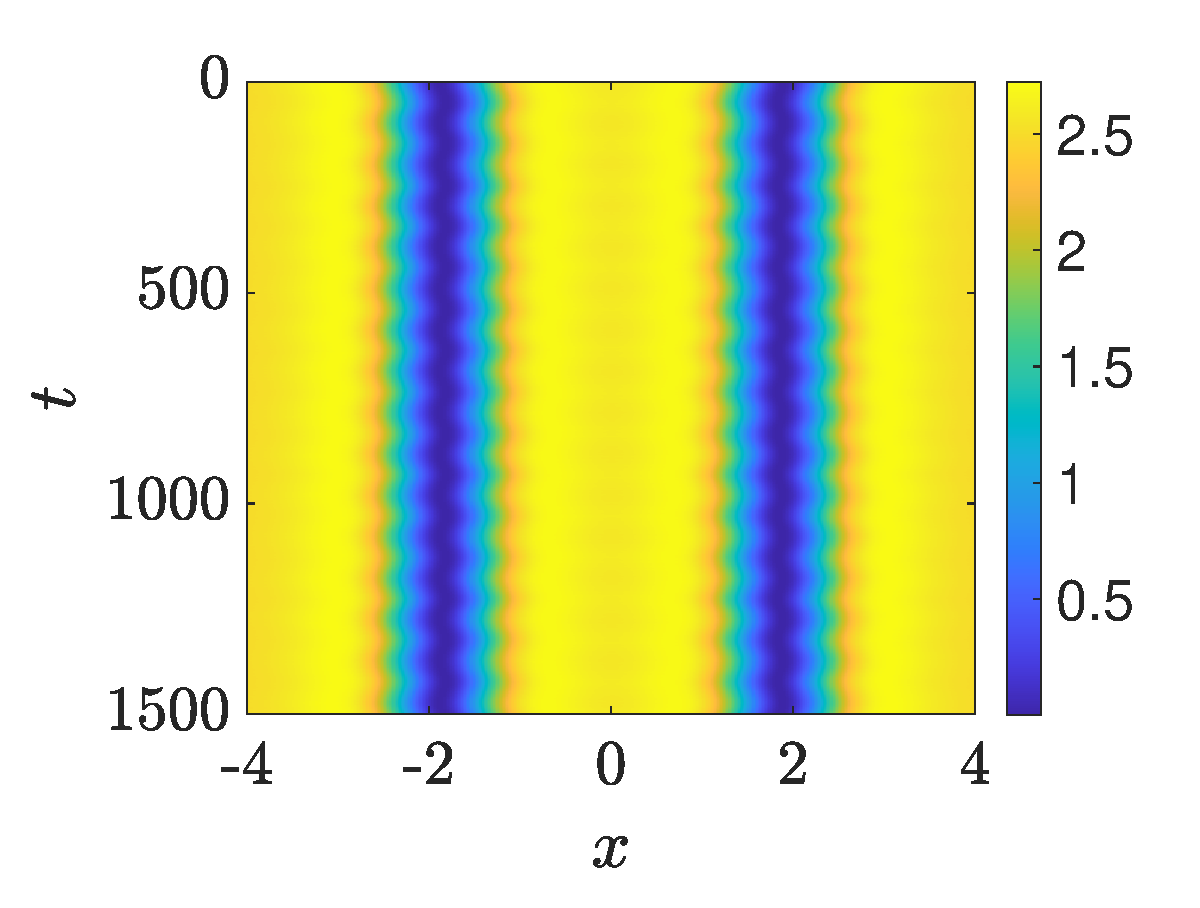
\includegraphics[width=5cm]{images/kak2colormap}
    \end{center}
    \caption{Top left: kink solution to NLS4 for $\beta_4>0$. Top right: two kink-antikink solutions; blue solution is unstable, red solution is spectrally neutrally stable. Bottom: time evolution of power of unstable (left) and neutrally stable (right) kink-antikink.}
    \label{fig:NLS4}
\end{figure}

Some recent work explores the $\beta_4 > 0$ parameter regime, in which the primary coherent structure is a ``kink'' (heteroclinic orbit) connecting two nonzero background states (\cref{fig:NLS4}, top left). Since the kink solution does not decay to 0, it is natural to pose the problem on a finite domain with Neumann boundary conditions. Kink-antikink solutions can then be constructed, in which a kink solution $u(x)$ and an anti-kink solution $-u(x)$ are spliced together. In contrast to the solitary wave solutions in the $\beta_4 < 0$ regime, it appears that the family of kink-antikinks alternates between unstable solutions (\cref{fig:NLS4}, bottom left), in which the kink centers repel each other when perturbed, and neutrally stable solutions (\cref{fig:NLS4}, bottom right), in which the kink centers exhibit oscillatory behavior. Both behaviors can be explained by the spectrum of the corresponding solutions. 

Another avenue of future research involves extending the model to incorporate terms characterizing Raman scattering, which leads to symmetry distortion and reduced pulse amplitude, as well as terms corresponding to gain and loss of energy. I am currently mentoring a graduate student who is exploring this problem. Another direction to explore would be to study a fourth order version of the generalized Lugiato-Lefever equation (GLLE), which is similar to NLS but contains a convolution term to model nonlocal effects.

\subsubsection*{Discrete systems}

I have also done work on discrete systems, including multi-pulses in the discrete nonlinear Schr\"odinger equation \cite{parker2020}, as well as multi-kinks \cite{ParkerSG} and multi-breathers \cite{Parker2022DKGbreathers} in the discrete Klein-Gordon equation. In both of these models, each lattice site is coupled to its two nearest neighbors via a discrete second difference operator, and the nonlinearity is centered at a single lattice site.
Future work includes extensions to models involving longer range interactions, as well as models such as Fermi-Pasta-Ulam-Tsingou (FPUT) lattices in which the nonlinearity involves off-site terms. Another class of natural extensions is to look at higher dimensional lattices. In two dimensions, there are many possible regular lattice models, including square, triangular, and honeycomb, and these different geometries may exhibit qualitatively different behavior. 


\subsection*{Topological photonics}

There has been much recent interest in the field of topological photonics, as experimental physicists and engineers have developed new techniques for controlling light propagation in photonic crystals and optical fibers. One specific application is light transmission through multi-core optical fibers. In particular, optical transmission properties can be tuned by introducing a twist to the fiber bundle. The propagation of light through a twisted optical fiber comprising $N$ waveguides arranged in a circle is described by the coupled mode equations
\begin{align*}
i \frac{d}{dz} c_n &= k \left(e^{-i\phi}c_{n+1} + e^{i\phi}c_{n-1}\right) + |c_n|^2 c_n &&  n = 1, \dots, N,
\end{align*}
where $z$ is the axis of propagation, $k$ is the strength of the nearest-neighbor coupling, and $\phi$ is a parameter representing the twist of the fiber. When the twist parameter $\phi$ and the number of fibers $N$ are related by $\phi = \pi/N$, I prove that there is a stable standing wave solution of the form $c_n(z) = a_n e^{i \omega z}$ which has a ``dark node'' with no optical activity opposite a ``bright node'' of maximum intensity \cite{ParkerTwist}. I also use an asymptotic approach to show that the same phenomenon occurs if the model incorporates a second-order temporal dispersion term \cite{ParkerSpatiotemporalTwist}. More recent work involves a model of a waveguide consisting of a square lattice of fibers, in which there are periodic variations along the waveguide axis causing the nearest-neighbor coupling to vary periodically in $z$ (\cref{fig:Rechtsman}, left) \cite{Mukherjee2020}. In particular, for any $z$, a waveguide is coupled to only one of its four neighbors. This configuration gives rise to localized periodic breather solutions, in which the bulk of the optical intensity is confined to a single square in the lattice but ``jumps'' around that square counterclockwise (\cref{fig:Rechtsman}, middle and right) \cite{Parker2021Floquet}. 
\begin{figure}
    \centering
    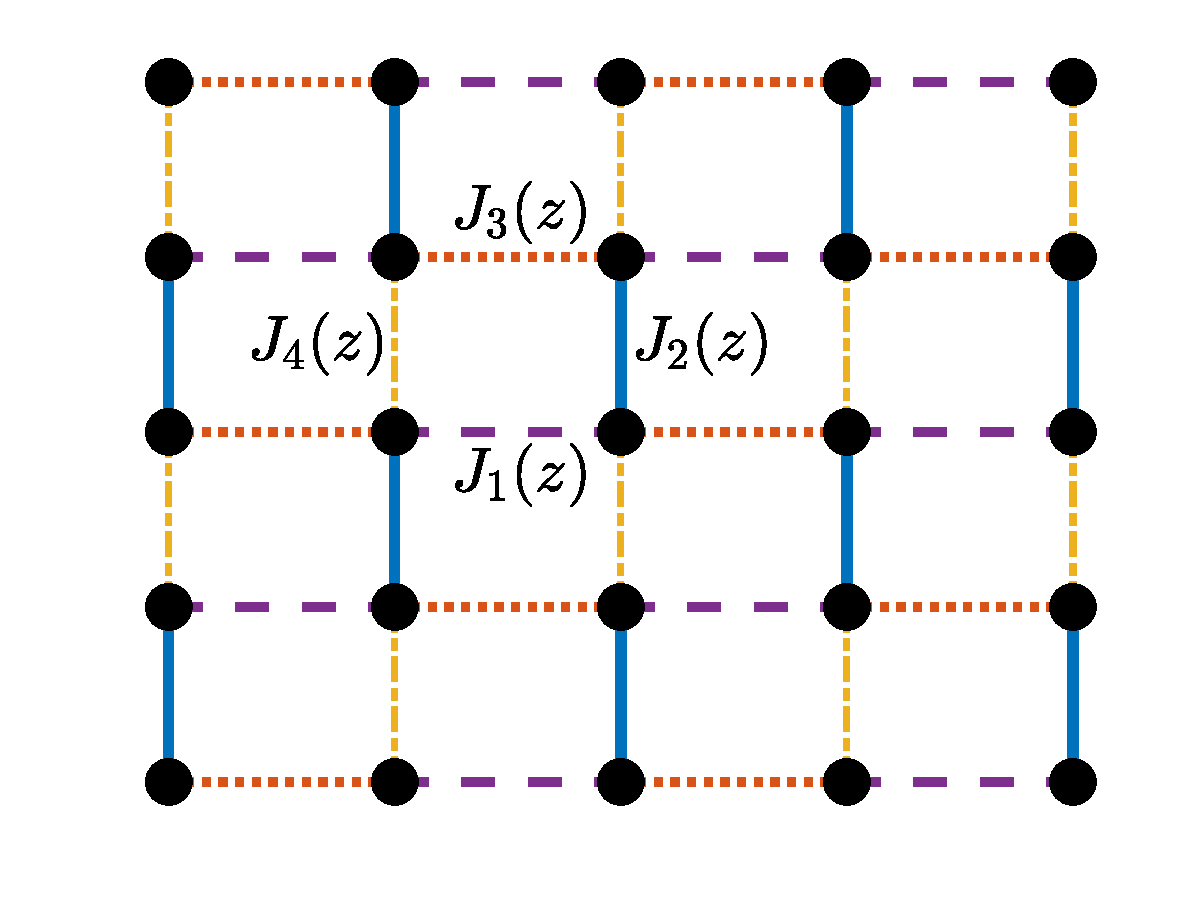
\includegraphics[width=4.5cm]{images/lattice.eps}
    % 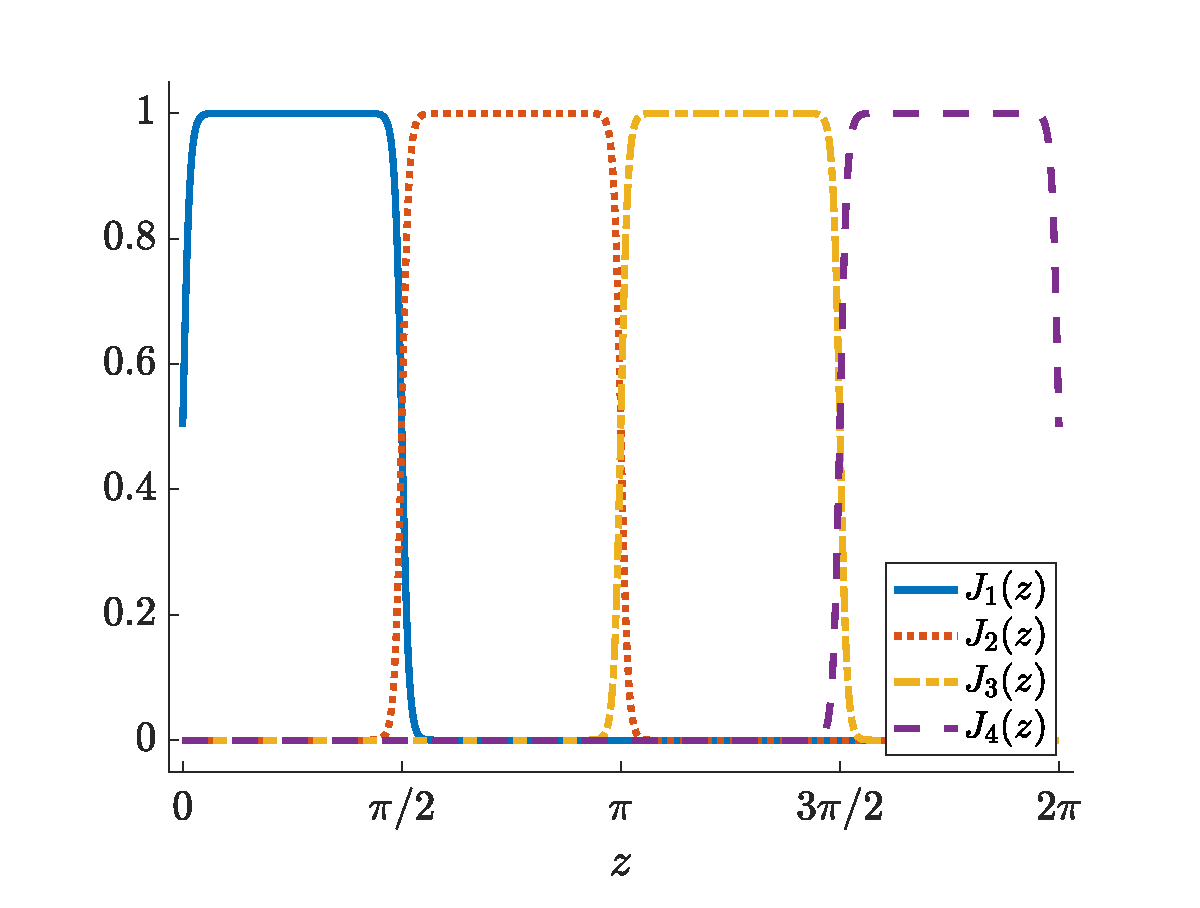
\includegraphics[width=7.8cm]{images/Jplot.eps}
    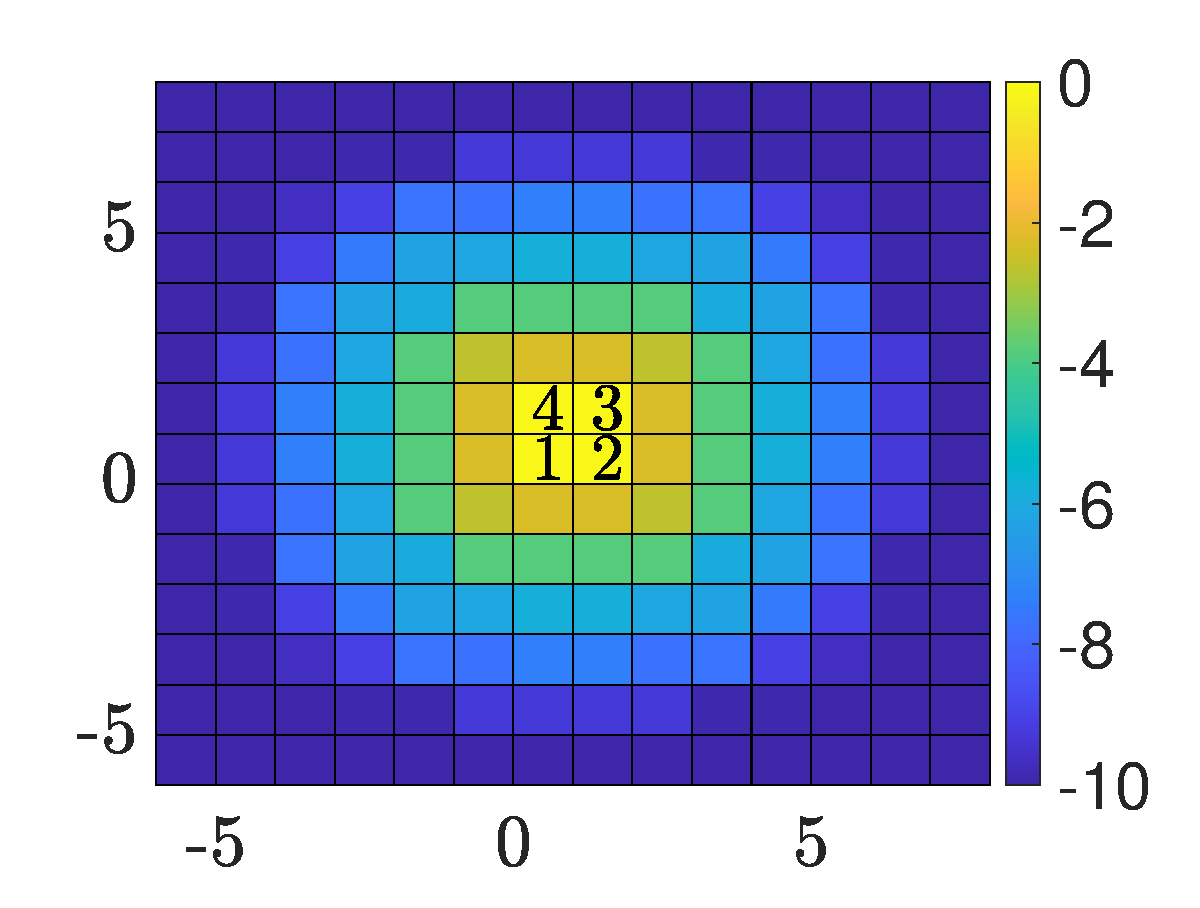
\includegraphics[width=4.5cm]{images/fundc1map.eps}
    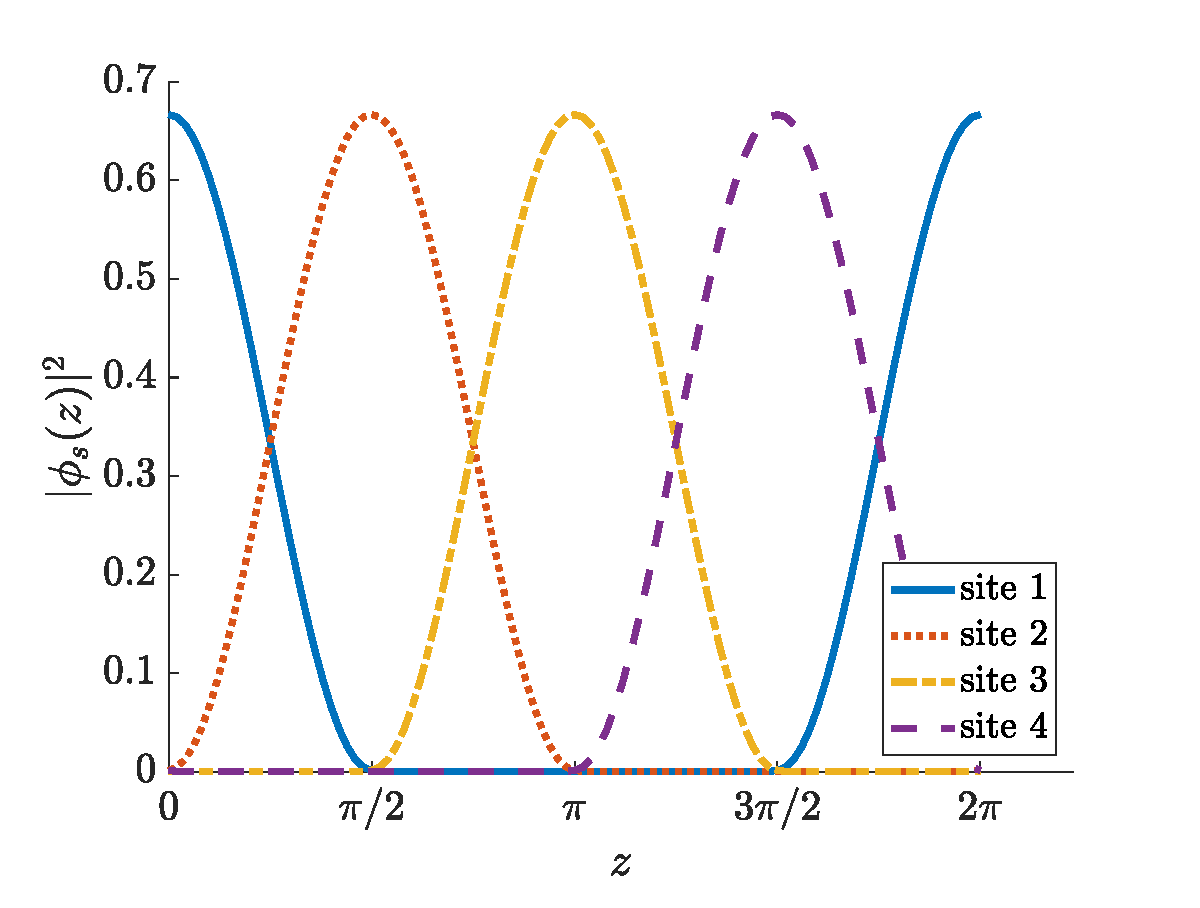
\includegraphics[width=4.5cm]{images/fundc1sol.eps}
    \caption{Schematic of square lattice with $z$-dependent coupling (left). At any value of $z$, only one of the four coupling functions $J_k(z)$ is nonzero. Log intensity of fundamental breather solution over one period, showing localization to a single unit square in lattice (center). Square intensity of fundamental breather solution on four sites of unit square over one period (right).}
    \label{fig:Rechtsman}
\end{figure} 
Future work involves studying solitons that ``hop'' between adjacent nodes in these optical lattices, and, in particular, the transition between stationary and ``hopping'' solitons.

\subsection*{Bifurcations in neural models}

Finally, some current work involves investigating bifurcations in a model of a neural network
\begin{equation*}
    \dot{\xvec} = -\xvec  + \frac{1}{\sqrt{N}} H\tanh (g \xvec),
\end{equation*}
where $\xvec = (x_1, \dots, x_N)$ represents the firing rate of each neuron in the network \cite{ParkerNeuro,Barreiro2017}. The network topology and neuronal connection weights are specified by the connectivity matrix $H$, and the individual neurons are connected using a sigmoidal hyperbolic tangent activation function. Adjusting the parameter $g$, which represents the global connection strength, leads to bifurcations, in which the stability and number of equilibrium points in the system change; periodic solutions may also emerge at these bifurcation points. The specific bifurcation structure depends on symmetries in the matrix $H$. 

For one example, suppose the neurons are grouped into two clusters, one containing excitatory cells and the other containing inhibitory cells. When $g = 0$, the origin is a stable equilibrium point of the system. As $g$ is increased, the origin loses stability in a symmetric pitchfork bifurcation (filled circle in \cref{fig:neuroBD}). Multiple branches of equilibrium points emerge from this bifurcation point due to the symmetries of $H$. As $g$ is further increased, there is a Hopf bifurcation (filled squares in \cref{fig:neuroBD}) on each branch of equilibria, after which point periodic orbit solutions are found. At a critical value of $g$, these limit cycles coalesce (dark band in \cref{fig:neuroBD}), after which point the system only has a single stable limit cycle. Future work with students includes exploring symmetries and bifurcations in the model resulting from other groupings of neurons, in particular hierarchical clustering models, as well as studying the effects of noise on the model. 

\begin{figure}
    \centering
    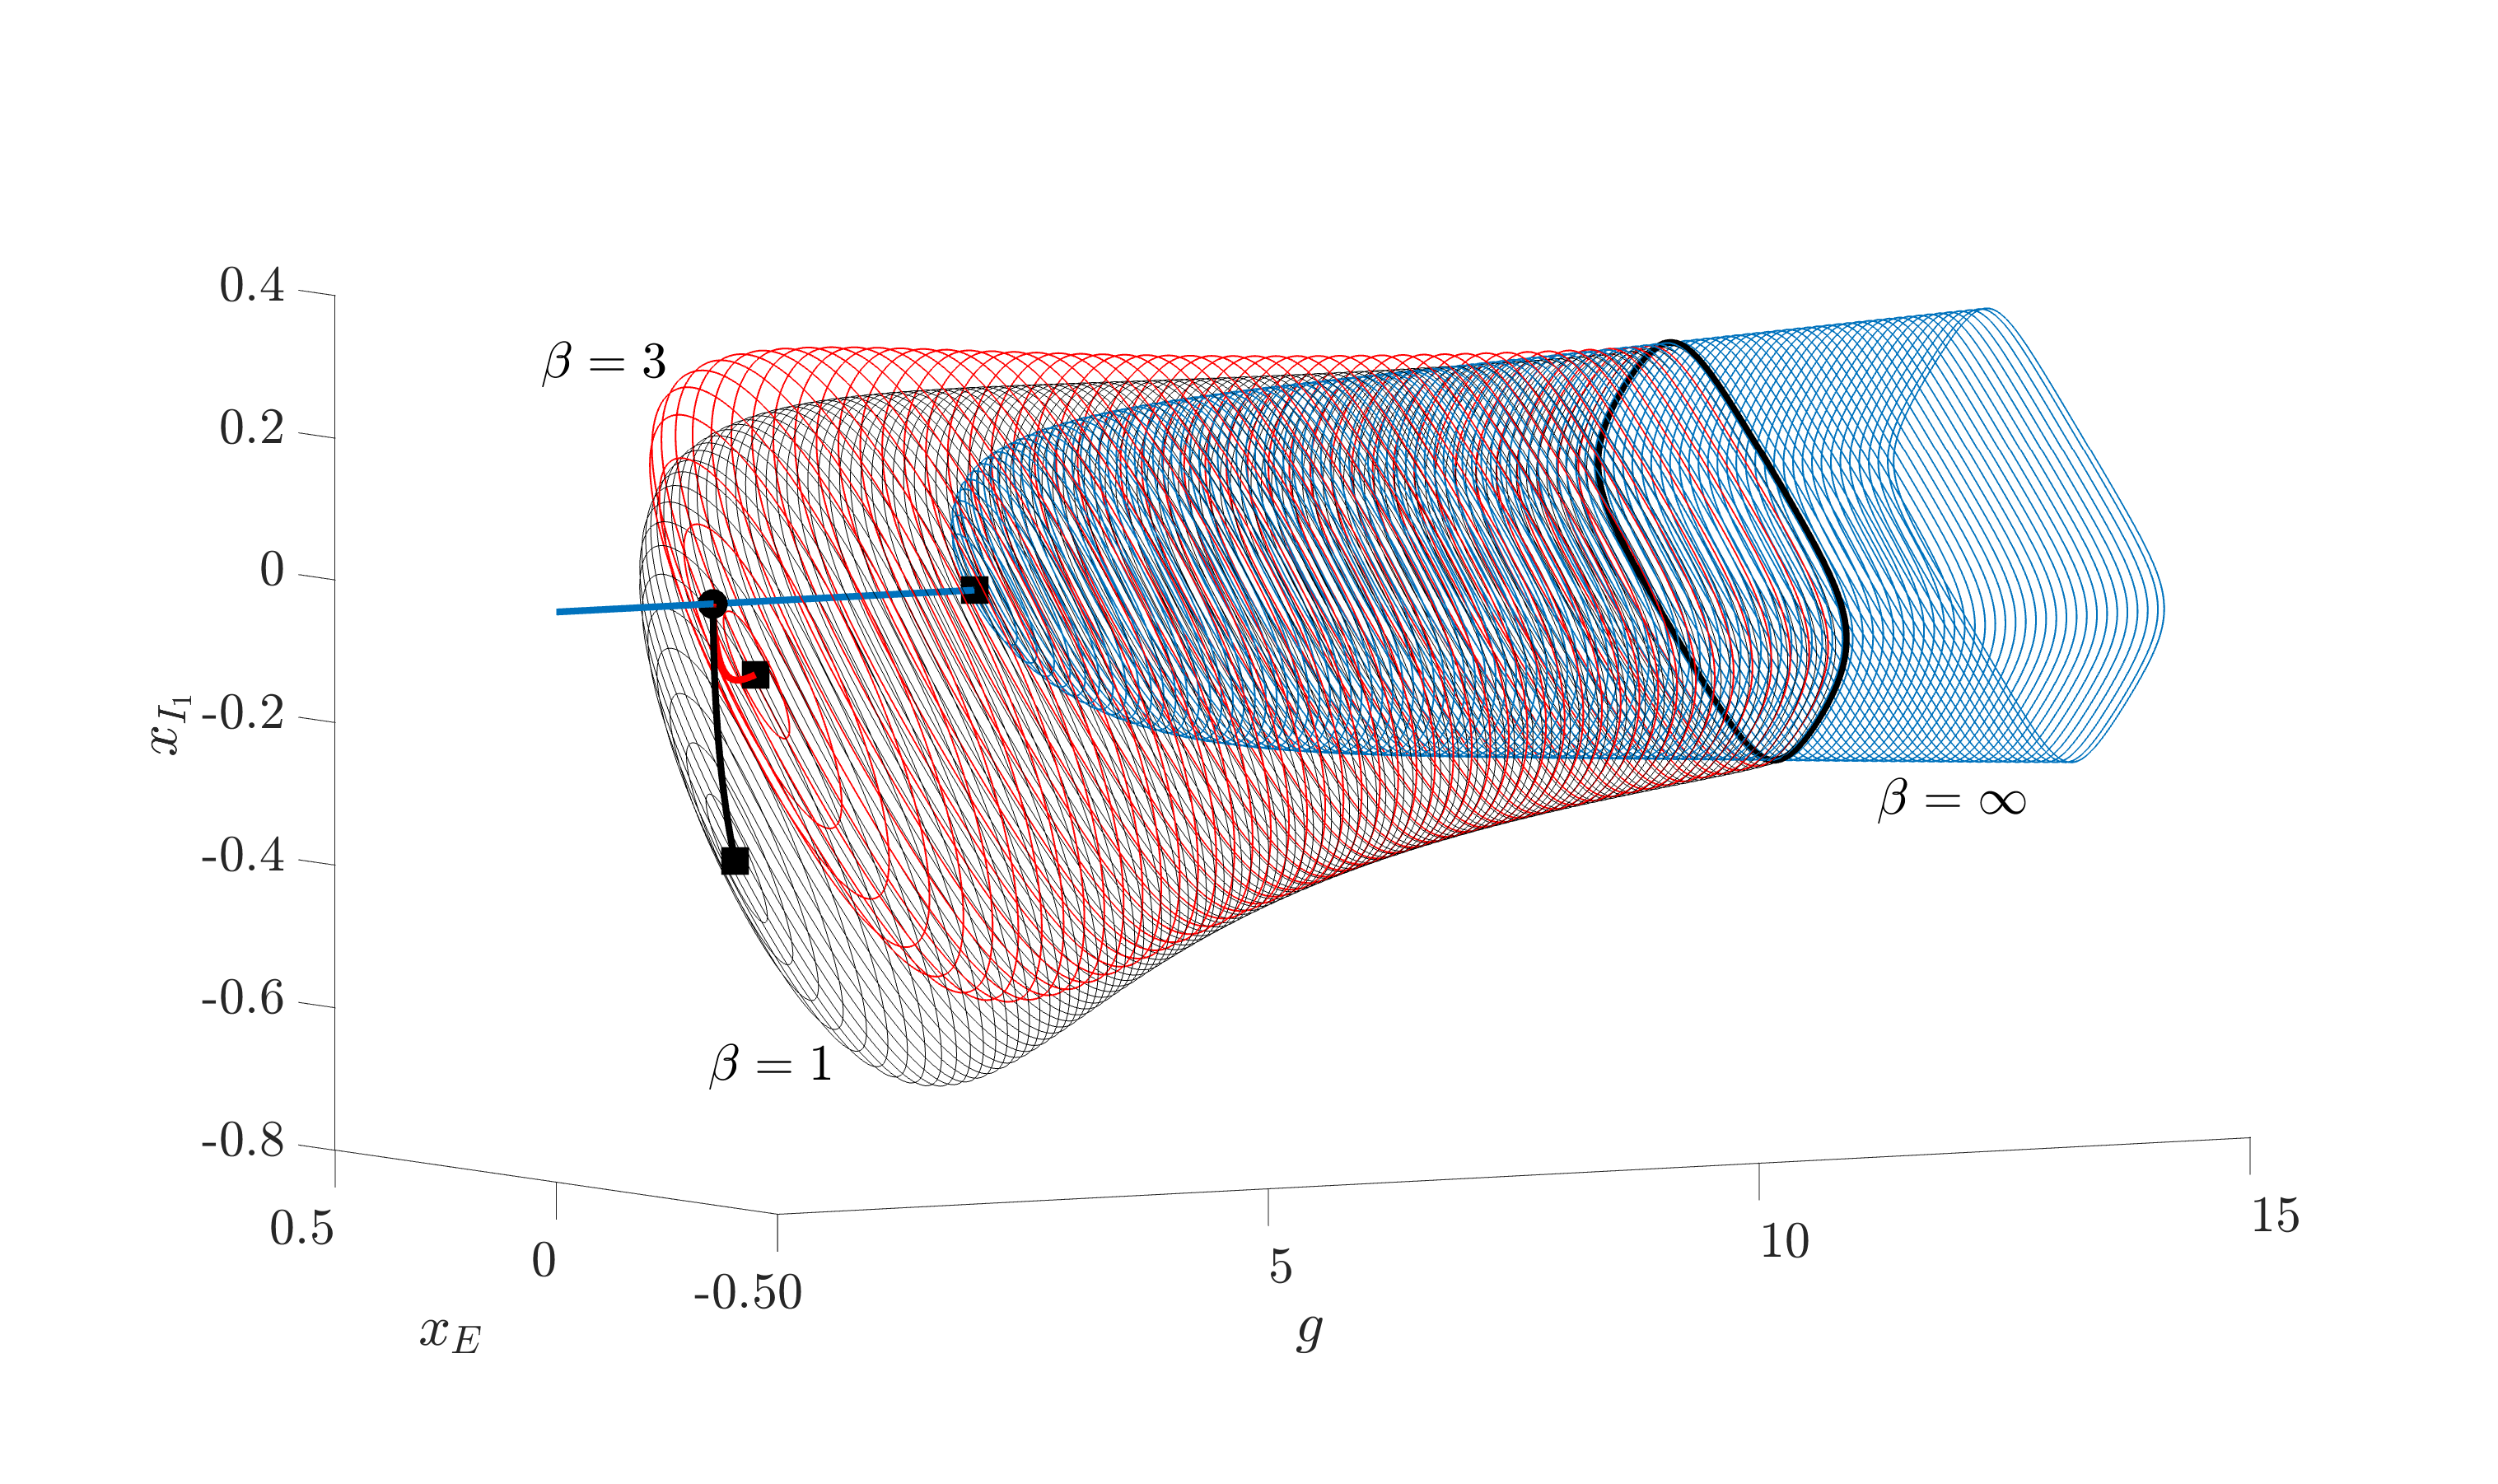
\includegraphics[width=12cm]{images/pitchbif.eps}
    \caption{Bifurcation structure of neural network model as the connection strength parameter $g$ is increased, showing fixed points (solid lines) and periodic orbits (rings). Symmetric pitchfork bifurcation indicated with filled circle. Hopf bifurcations indicated with filled squares.}
    \label{fig:neuroBD}
\end{figure}

\subsection*{Future work}


\bibliographystyle{amsplain}
\footnotesize{ \bibliography{researchstatement.bib} }

\end{document}
